\documentclass[a4paper,11pt,uplatex]{jsarticle}


% 数式
\usepackage{amsmath,amsfonts}
\usepackage{bm}
\usepackage{physics}
% 画像
\usepackage[dvipdfmx]{graphicx}
\usepackage[dvipdfmx,colorlinks=true,linkcolor=blue]{hyperref}
\usepackage{pxjahyper}

\begin{document}


\section{導入}
\subsection{ハイパー核質量分光}
Λ粒子はu,d,sクォークからなるハドロンである。\\
Λ粒子を内部に含む原子核はΛハイパー核と呼ばれる。\\
Λ粒子と核子間相互作用を決定することは一般のハドロン間相互作用の理解にも重要である。\\
ハイパートライトンは陽子、中性子、Λ粒子一つずつからなる原子核で、
\subsection{崩壊パイ中間子法}
崩壊パイ中間子法は2010年代にドイツのマインツ大学マイクロトロン(MAMI)で開発されたハイパー核質量分光法である。
電子ビームで生成したハイパー核が破砕化し、目的のハイパー核が標的中で静止し2体崩壊する反応を検出する。
静止かつ2体崩壊という崩壊の特徴により放出されるパイオンの運動量は単色的であるため、高い質量分解能が期待される。
MAMIの持つ高分解能運動量スペクトロメータはこのパイオン運動量を10 keV以下の分解能で検出可能である。
これによってハイパー核の質量やそこから計算されるΛ粒子の結合エネルギーも10 keV以下の精度で検出が可能となる。
この高分解能は他のハイパー核質量分光法にはない崩壊パイ中間子法の特徴である。
\subsection{系統誤差}
しかしながら、スペクトロメータの較正誤差がs00 keV程度と大きいことが実験全体の誤差を制限していた。
電子の弾性散乱実験で得られるピークを計算と比較することで運動量較正を行っているが、入射電子ビームエネルギーの絶対値決定精度が100 keV程度と大きいことで
計算される運動量の不確かさが100 keV程度ある。これによって運動量較正精度が100 keV程度に制限されている。
すなわち、スペクトロメータの較正精度を10 keVに向上させることで、実験全体の誤差を100 keVから10 keVに向上させることができると考えられる。
そのための一つの方法として、我々は電子ビームエネルギー絶対値決定精度を向上させる手法の開発に取り組んできた。
\subsection{Undulator Interferometry}
電子弾性散乱位に用いる200 MeV領域の電子ビームを測定する手法は限られている。
我々は2016年からアンジュレータによる放射光を用いた電子ビームエネルギー較正手法の開発に取り組んできた。
\subsection{Calibration beamtime}
Method\\
Analysis\\
Validation\\

\clearpage

\begin{figure}[tb]
  \centering
  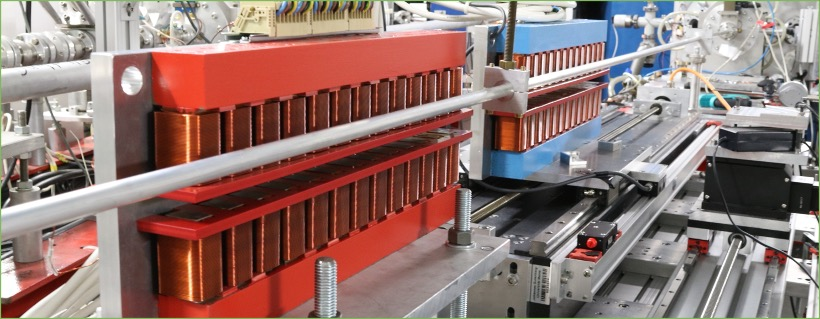
\includegraphics[width=0.8\linewidth]{image/1-1.jpg}\\
  \caption{サンプルの図}
  \label{sample_image}
\end{figure}

\begin{itemize}
  \item a
\end{itemize}
\begin{enumerate}
  \item b
\end{enumerate}

\begin{align}
\frac{1}{2} = \qty(\frac{1}{3}) + \qty{1}\Sigma
\end{align}
\end{document}